\section*{}
In Part \ref{part:related_work}, we have seen the various facets of password-based authentication problems. However, a few central problems remain understudied and deserve further attention: has user education been successful in the past decade and in which ways? How severe is the threat of password reuse and are there ways to detect it and to mitigate risks? 

The next chapters shed light on these aspects of the problem space of usable password security. 

\chapter[Mental Models of Password Strength]{Mental Models of \\
	Password Strength}\label{chap:pasdjo}

This chapter reports on findings published at OzCHI 2017 \cite{Seitz2017PASDJO}. The insights and data are put into context and extended with additional analyses. 

\section{Background and Context}
% Assumption: Users don't know how to create strong passwords
Users create passwords on a regular basis. As discussed in Chapter \ref{chap:rw:user_perspective}, previous research indicates that users most commonly resort to weaker passwords that are easy to remember. In case the account value is higher, however, it is suspected that users invest more effort into creating a stronger password. Password meters are helpful in this context \cite{Egelman2013DoesMyPasswordGoUpToEleven}. Yet, even these stronger passwords are often ineffective against sophisticated guessing attacks, so it stands to reason that users have a subpar mental model of what makes a strong password. This has been a commonly accepted assumption \ar but it oversimplifies the state of affairs. 

% perceptions and mental models change over time. 
First, mental models change over time -- both on a micro- and a macro-scale. At micro-scale, it is evident that the first passwords are chosen in teenage years and without much care for security \cite{VonZezschwitz2013SurvivalShortest}. Over time, users are exposed to password advice and educational nudges: popular news portals regularly publish new articles that report on data breaches or warn about risky online behavior. This and incidents in one's own social network \cite{Stobert2014PasswordLifeCycle} raise awareness about the topic and can spark plans to behave differently in the future. Moreover, registering with multiple services increases the likelihood of facing different password policies and password meters which nudges users to reflect on their password choice. Potentially they might also alter their mental models if feedback and policy instructions are well-designed \cite{Shay2015SpoonfulOfSugar, Ur2017DataDrivenPWMeter}. The literature already has some evidence that, overall, password behavior has positively changed in the past few decades \cite{Riley2006WhatUsersKnowWhatTheyDo, Schneier2006RealWorldPasswords}. 

% education seems to have paid off.
Zooming out to the macro level, efforts to educate users may have already paid off. In the early days of research in Usable Security, often the user was seen as the ``weakest link'' in a secure system \cite{Adams1997MakingPWsSecureAndUsable, Sasse2005UsableSecurityPosition}. When Florêncio and Herley conducted their large-scale study in 2006/2007, they saw relatively low-entropy passwords, but higher-value accounts were a bit better protected. However, in 2015 Ur \etal found that users' mental models had become better which allowed them to create stronger and memorable passwords \cite{Ur2015PWCreationLab}. A year later, they presented an in-depth analysis of the perceptions of password strength \cite{Ur2016PerceptionsPassword}. They found that for the most part, participants in their online-study were capable of identifying the factors that add to password strength. Shay \etal already used ``perceived strength'' as a proxy metric \cite{Shay2015SpoonfulOfSugar}, and it seems this is a better approach than one might think. For a few notable exceptions, though, certain password characteristics fooled participants. Ur \etal argue that errors in mental models about strength arise from false understandings of attackers. Consequently, it would be necessary to shift education from password strength towards attackers, because users already have a fairly accurate understanding of strength. 

%TODO maybe add a third argument here (perceptions might be the)
%or: Florencio / finite effort stating that users are smarter than we might think
Florêncio \etal put forward a formal model as to why users behave insecurely. Their central argument is that it is inevitable to choose weak passwords for some accounts and that users are well aware of their behavior. Yet, if users have a faulty understanding of password strength then the selection process is biased. In the case of users also showing the overconfidence bias, where people are subjectively more confident in their abilities and judgments than the objective accuracy of the judgments \cite{Simonson1989ChoiceBasedOnReasons}, this could indeed lead to considerable risks.  %TODO go on. 

% summary: perceptions are still understudied 
In summary, having a clear mental model of what makes for a strong password is essential to make the decision whether to use one or not. While there are initial results, the perceptions of these factors is still understudied to this point.

\subsection{Research Objectives}
In this project, I wanted to investigate the origin of weak passwords. I challenged the folk model that users behave insecurely due to their lack of knowledge (as proposed by \ar). If users are able to identify weak and strong passwords, it is fair to assume they can select appropriately strong passwords depending on the situation. With this knowledge, we can rethink password feedback. As pointed out above, current password meters and verbal feedback might be ineffective because if the majority of users is aware of the strength of their password. Instead, feedback could be framed around re-use or attack models. Solidifying evidence from related work with a novel study approach was a fruitful step towards making a holistic design recommendation regarding the feedback aspect of password support systems. 

%\begin{itemize}
%	\item find more evidence of password misconceptions
%	\item educate users at the same time? --> problematic because we didn't really focus on it and left it to the users to figure out how it works.
%\end{itemize}

\subsubsection{Research Questions}
The specific research questions for this project were as follows:
\begin{itemize}
\item[RQ1] How well can users identify weak and strong passwords?
\item[RQ2] What types of password topologies lead to the most errors?
% maybe can we corroborate Ur \etal's findings in a cheaper and more engaging way? 
\end{itemize}


%\section{Related Work}

\section{Approach: PASDJO - The Password Game}
To evaluate (in)accuracies in mental models about password strength, I chose to have users rate passwords similarly to the study task in Ur \etal's study \cite{Ur2016PerceptionsPassword}. In their presentation at CHI 2016, they challenged the audience which sparked the idea of making a game out of this task. To open the game to a large audience, I decided to implement it as a web-application that runs in any web browser on various platform. 

\begin{figure}
	\centering
	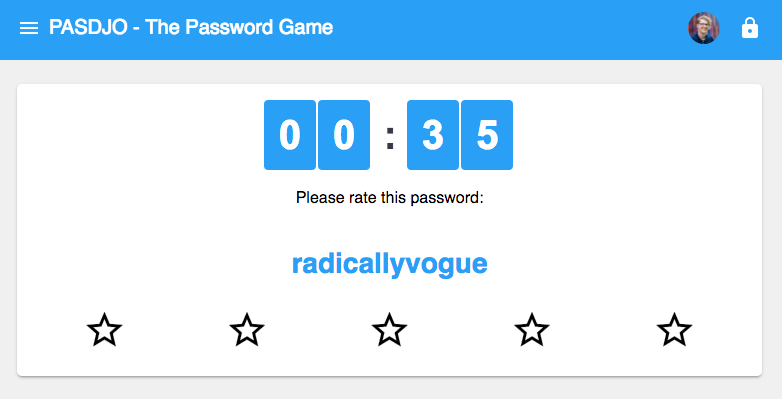
\includegraphics[width=0.75\textwidth]{pasdjo/radicallyvogue}
	\caption{\label{fig:pasdjo:radicallyvogue}}
\end{figure}

\subsection{Game Mechanics and Design Elements}
The game is relatively simple: Players judge how strong or weak a given password is. They receive points by accurately estimating the strength of a given password on a scale from 1 (weak) to 5 (strong). The game follows similar design strategies for the password topologies as the Ur \etal's online study, but passwords are either randomly taken from large dictionaries or generated on the fly. To induce intuitive estimations, a time-limit is enforced while a ``highscore'' acts as incentive to estimate as accurately as possible. To reach higher scores, one has to judge as many passwords as possible in 60 seconds. 

\subsubsection{Scoring and Metrics}
A crucial point of the game is how the passwords are rated objectively. Here, we rely on the zxcvbn library\footnote{\url{https://github.com/dropbox/zxcvbn}} (described in detail in Section \ref{sec:rw:pw_strength_metrics}) because it is highly reliable and straightforward to use on a web page. It also comes with a number of word lists that are helpful to implement different scenarios, respectively conditions. Beside the guess-number metric, zxcvbn also scores passwords on a scale from zero (weak) to four (strong). We translate this scale to one star (weak) to five stars (strong) in the game. 

For a correct estimation, a match between zxcvbn score and the player's score, a player is awarded 100 points. The difference between the user's rating and the zxcvbn score is the \textbf{\textit{deviation}} ($D$). A player's rating can deviate by at most four stars, e.g. if they rate a five-star password with a score of one and vice versa. In that case, the player should not get any points, but in all other cases, the player is still awarded fewer points. For each integral deviation in either direction there is a penalty of 25 minus-points (maximum of 100 points, at most 4 errors, which leads to $100 / 4 = 25$). The points of the estimations are summed up and build the \textbf{\textit{achieved}} score ($A$). As an overall accuracy measure, at the end of the game we calculate the ratio of achieved and possible points and display it as percentage ($P$). The game thus implements the following scoring function, where $U$ is the user's estimation on a scale from 1 to 5, $Z$ is the zxcvbn score on the same scale, and $n$ is the number of passwords a user has rated within the time limit. 

\noindent The scoring function takes an array of user ratings and zxcvbn scores for $n$ passwords and returns a vector consisting of the achieved points $A$ and accuracy metric $P$.
\[
f([(U|Z)_1, ..., (U|Z)_n]) = (A|P)
\]

\noindent For each estimation the deviation from the zxcvbn score is calculated.
\[
D_k = U_k - Z_k\\
\]

\noindent The total achieved points are the sum of the achieved points per round. Each round takes the 25 point penalty into account. If $|D_k|=0$, the player gets the full 100 points per round.
\[
A = \sum_{k}^{n} 100 - (|D_k|*25) \\
\]
\noindent Finally, the accuracy is the fraction of achieved and possible points. 
\[
P = \frac{A}{n * 100}\\
\]

The score and accuracy are displayed to the users once the game is finished, see Figure \ref{fig:pasdjo:feedbackscreen}.

\begin{figure}
	\centering
	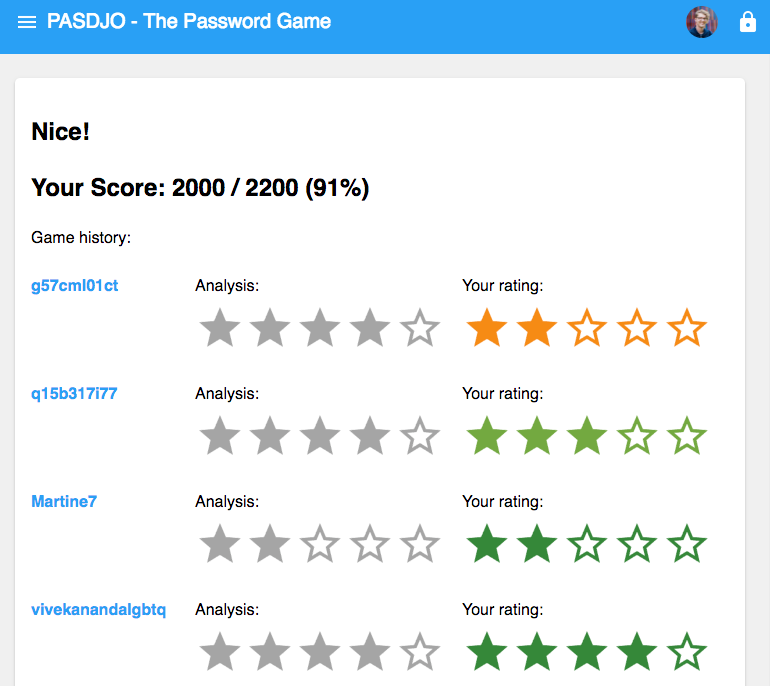
\includegraphics[width=0.75\textwidth]{pasdjo/feedbackscreen}
	\caption{\label{fig:pasdjo:feedbackscreen}}
\end{figure}

\subsubsection{Persuasive Design Elements}
We used a number of persuasive techniques (see Section \ref{sec:rw:persuasive-interventions}) in the design of the game. Most of them relate to the \acrlong{PAF} \cite{Forget2007PersuasionEducationSecurity}. First of all, we lower the barrier to play the game through \textit{simplification}: the task is immediately clear and does not require special skills. Since one round only takes sixty seconds, it is easier for users to \textit{commit} to finish the game. The feedback screen uses positive \textit{language} to create the notion of a \textit{social interaction}, which also serves \textit{self-monitoring}. Also, feedback and points serve as \textit{reinforcement} for correct ratings, i.e. a subtle form of \textit{conditioning}. Moreover, the user interface is \textit{tailored} to the user, as they can see their own previous scores. Players can also create an account through Google-federated \gls{SSO}. If they log in, their profile picture and a personal greeting \textit{personalize} their experience. Through the player's eyes, the game's strength ratings are ``right'', which can be attributed to the \textit{authority} principle. Finally, the game leverages the \textit{goal-gradient effect} by giving the player small amounts of points even for inaccurate estimations. At the end, the player receives a score that seems improvable through playing another round. 

\subsection{Password Generation and Study Conditions}
\makeatletter
PASDJO initially had four different password types that act as levels of the independent variable: Common passwords, mangled passwords, passphrases, and random passwords. During gameplay, the condition for the next password was selected at random. The following paragraphs depict the conditions in detail. 

%%%% COMMON
\paragraph{Common passwords: } We take the word lists that come with the zxcvbn library. One of these lists contains 47023 leaked passwords ordered by frequency, from which we randomly pick one for this condition. The data stems from breaches of user databases at RockYou, Yahoo and Xato \cite{Wheeler2016zxcvbn}. All passwords are lower-case and can be considered weak, because they are usually amongst the first attempts in a guessing attack \cite{Ur2015MeasuringRealWorldAccuracies} unless the adversary launches a targeted attack where personal information plays a more important role. Zxcvbn rates the top 1000 passwords with a score of 1 (e.g. ``12345'', ``password'', ``monkey''), and the remaining passwords are scored with two stars (e.g. ``iloveyou2'', ``skywalker'', ``apollo13''). It is worth noting that many of these passwords would not be accepted anymore by websites as common policies demand at least 8 characters (see Chapter \ref{chap:policies-reuse}), which RockYou and Xato did not enforce at the time. %TODO the last remark could go somewhere else. 

%%%% MANGLED
\paragraph{Mangled passwords: } For the mangled password condition, we take the same list of the top 47023 passwords, but we algorithmically substitute certain characters. The substitutions look like ``leet''  / ``l33t'' speak, which is a typical way to try to increase password strength \cite{Das2014TangledWeb, Mazurek2013Measuring}. For instance, an ``a'' is replaced by an ``\@'', or an ``s'' is substituted with the dollar sign ``\$''. Also, random characters are transformed to uppercase. To allow recognizing the original word, we only mangle up to 30\% of the characters of the password. Since we only use substitutions that zxcvbn recognizes, mangled passwords mostly receive a score of two. However, in rare occasions, they occupy the full range, i.e., ``p@ssw0rd'' (1), ``b0n3he@d'' (2), ``fireFI9hter'' (3), ``123qaz456w\$x'' (4), ``123Q@z4s6w\$x'' (5). 

%%%% RANDOM
\paragraph{Random passwords: } We implemented a simple string generation algorithm to create random passwords. They are lowercase alphanumeric passwords containing letters from the German alphabet, i.e. [a-z0-9äöü]. Zxcvbn consistently gives them a score of four, which makes them easy to rate. In a real-world attack they can only be brute-forced \cite{Florencio2014AdministratorsGuide, Wheeler2016zxcvbn}.

%%%% PASSPHRASES
\paragraph{Passphrases: } We combine two entries from the English Wikipedia index to create a passphrase (also shipped with zxcvbn). The words were required to be between 4 and 11 characters long. This restriction leads to a dictionary size of 27202 entries. Thus, there are $27202^2 \approx 10^9$ possible combinations, which is unpredictable enough to withstand online guessing attacks. This is reflected by the rather high scores: zxcvbn gives passphrases mostly a score of three or four, e.g. ``armedtamils'' (3), ``boostedeuros'' (4). If the words appear in other dictionaries, e.g. the ``TV subtitles'' word list, they are more likely to result in a score of three. However, for a user it is not straight-forward to tell whether a passphrase scores three or four points, which makes this condition harder to get right. The game is expected to benefit from this element of \textit{unpredictability}, which is one of the eight cornerstones of gamification according to Chou \cite{Chou2015Gamification}.

\vspace*{2ex}
For the remainder of the chapter we refer to these four condition as ``Common'', ``Mangled'', ``Random'', and ``Passphrase''.

\subsection{Benefits and Shortcomings of the Game-based Approach}\label{sec:pasdjo:beneftis_shortcomings_method}
Since the game was deployed publicly, the method can be denoted as an unsupervised in-the-wild study. This approach has certain benefits and shortcomings as discussed in the following. 

\subsubsection{Benefits}
\textbf{Easy collection of multiple data points per user} The game can be played over and over. A survey could also be taken multiple times, but most of the time this is not desirable. If the study is done via MTurk this would mean that people would be paid each time which drives costs.

\vspace*{1ex}
\noindent\textbf{Possibility to provide feedback} After the game, the players can review their ratings and find out how they performed. In a study, implementing such a feedback loop is much more complicated and often impossible with current survey tools. Hence, a debriefing step is required, but it's difficult to tailor it to the individual participant.

\vspace*{1ex}
\noindent\textbf{Randomization and password space} Ur \etal's study was designed well in that it tested a wide range of password characteristics and there were multiple options per condition. However, the options were predefined by the researchers and limited in that sense. In our case, we can pick passwords from much larger word-lists at random and use algorithms to randomly adjust certain characteristics. This allows for higher internal validity of the data collection.

\vspace*{1ex}
\noindent\textbf{Intrinsic Motivation} Participants in an online survey often receive an incentive to participate. In an \gls{mTurk}-studie each participant receives a small amount of money. Contrarily, there is no extrinsic incentive to play PASDJO. 

\vspace*{1ex}
\noindent\textbf{Intuition} The game uses time pressure to induce intuitive responses. Thus, if playing fast enough, we expect to measure System 1's responses instead of System 2 \cite{Kahnemann2011FastAndSlow}. This is vital because password selection is often a System 1 process, i.e. an intuitive and automatic. In an online survey, the participants can take as much time as they'd like to reason about their response. However, this is a hypothetic benefit that needs further empirical evidence. 

\subsubsection{Drawbacks}
The game approach to collecting password strength perceptions naturally entails drawbacks, too. First and foremost, we do not collect demographic data. In a survey, it is common practice to include questions about basic demographic information. If we included such questions as part of our game, we might have scared off users and damaged persuasive strategies. Thus, the collected data stems from an unknown population, which is a limitation. %TODO maybe add a sentence why it is still good to collect the data.

Furthermore, the lack of demographic data also makes it hard to track usage across multiple devices. The same player could first get in touch on a desktop and then later decide to keep playing on their mobile. Allowing users to log in and synchronize their game history can mitigate this problem to some degree.

Last, ethically running password studies (see Section \ref{sec:rw:methodology}) demands that participants be debriefed appropriately. In our case, we provide a separate ``About'' page that is accessible from anywhere in the app. The information on the about page points out that users should refrain from using the generated passwords as their own and that our strength estimation is only an estimate. Nevertheless, it requires that users seek this kind information, which -- realistically -- only few people might do. Therefore, as a small encouragement to read it, we require users to confirm a consent-dialog that also points them to the about page. 

\subsection{Implementation}
For the implementation, we used modern web technologies to create a state-of-the-art user experience. The front-end uses the polymer library\footurl{https://www.polymer-project.org/}{22.01.2018}. \textit{Custom elements}, which were recently standardized in the WebComponents standard\footurl{https://www.webcomponents.org/specs}{22.11.2018}, serve to separate concerns through encapsulation. On the back-end, we rely on the Firebase platform\footurl{https://firebase.google.com/}{22.01.2018}. It allows setting up an easy and secure authentication, respectively authorization, workflow. Moreover, the data is stored in a \textit{real-time-database} that uses fast web-socket connections to synchronize data between client and servers.

\begin{figure}[!tbp]
	\centering
	\begin{subfigure}[t]{0.3\linewidth}
		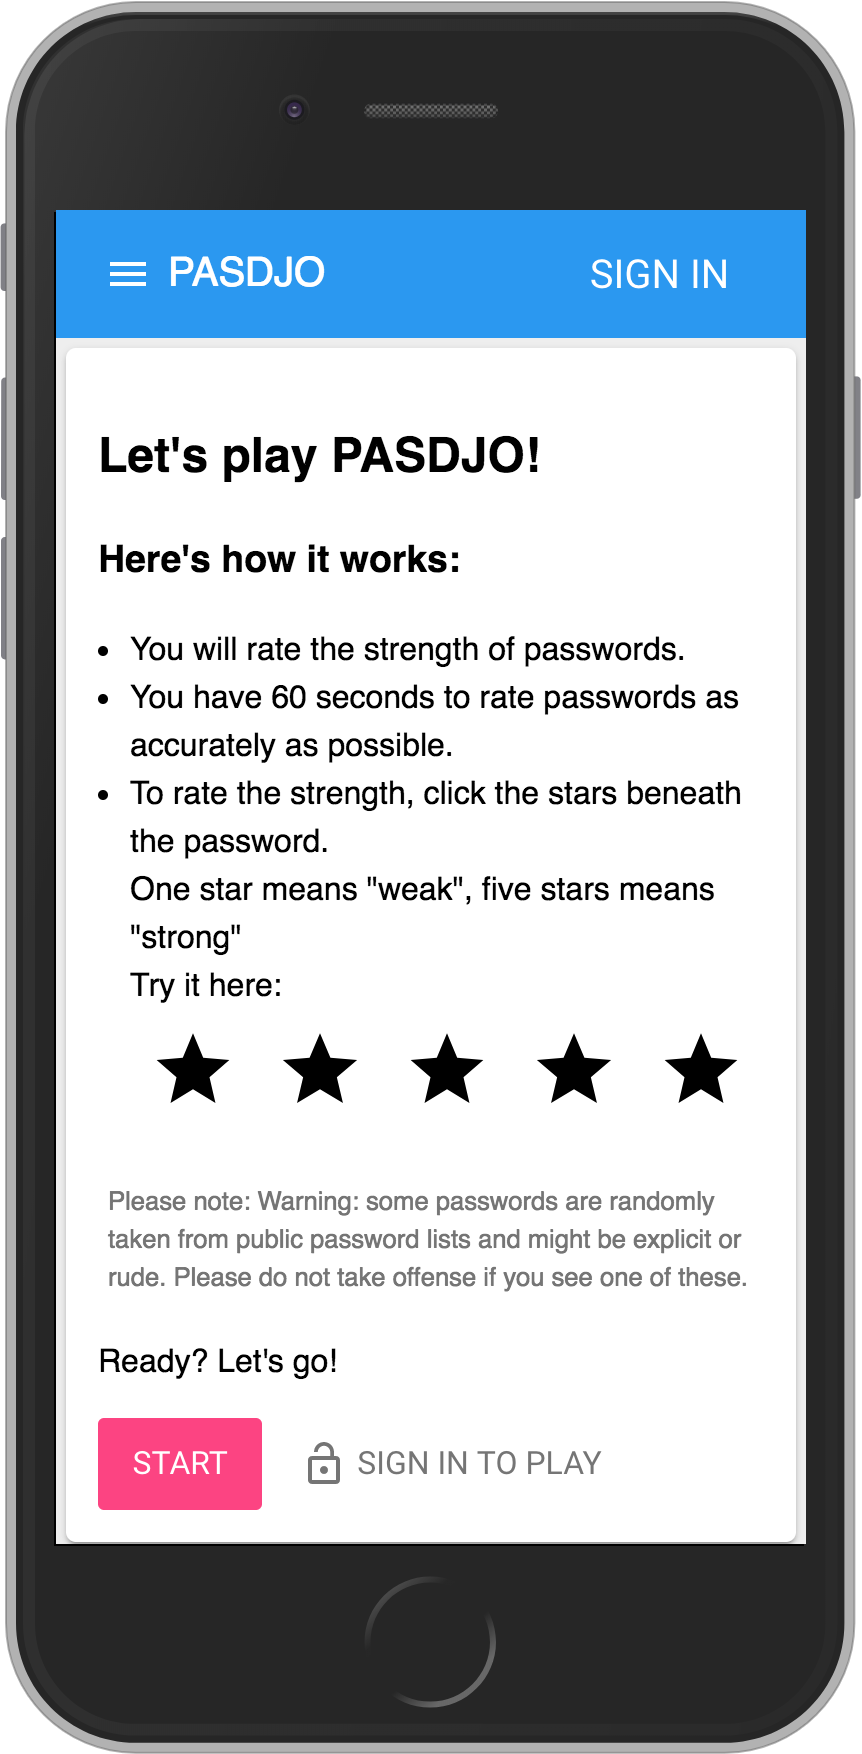
\includegraphics[width=\textwidth]{pasdjo/welcome-iphone-frame}
		\caption{\label{fig:pasdjo:welcome-screen}Welcome screen for anonymous users. The game is briefly explained and the users can try the rating interface (stars)}
	\end{subfigure}
	\begin{subfigure}[t]{0.3\linewidth}
		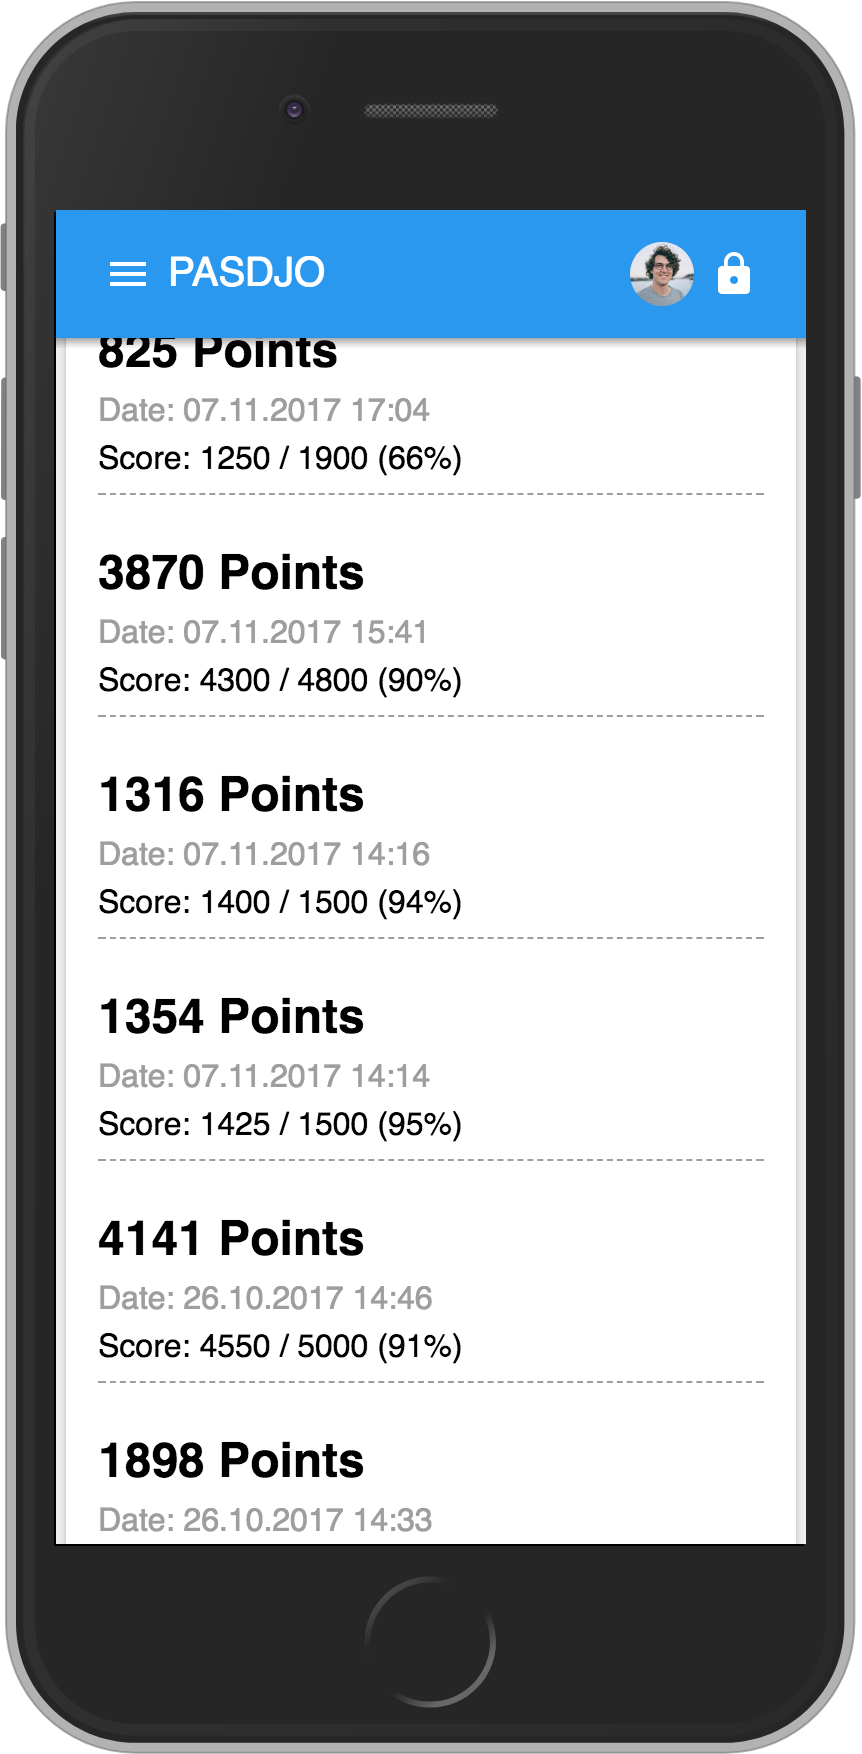
\includegraphics[width=\textwidth]{pasdjo/history-iphone-frame}
		\caption{\label{fig:pasdjo:history-screen}Users can browse through past games. The updated version visualizes the scores in a line chart (not displayed)}
	\end{subfigure}
	\caption{\label{fig:pasdjo:welcome-history}Key screens in the user interface.}
\end{figure}

We took user experience heuristics to design the game for a large audience. Among others, we based our solution on the Progressive Web-App heuristics\footurl{https://developers.google.com/web/progressive-web-apps/checklist}{22.01.2018}, which we hoped would lower the barrier to engage with the game. Since we expected many people from Germany would play the game, the interface is fully localized. Depending on the browser language, it automatically picks the preferred language. Moreover, the interface is responsive to different screen sizes to provide a seamless experience. We chose a short URL \url{pasdjo.de} to facilitate visiting the website from mobile devices where typing is cumbersome. Upon visiting the web page, a welcome screen briefly explains the rules (see Figure \ref{fig:pasdjo:welcome-screen}). As part of our onboarding process, we give users the opportunity to try out the rating interface, so they can get comfortable even before they play for the first time. For mobile users, we had to ensure that the game loads quickly. This is challenging, because we have to transfer a number of word lists to generate the passwords randomly. Therefore, we used a lazy-loading design pattern to render the UI first and load data in the background. At the same time, we minimize and compress the source files to reduce data transfers. The first page load consumes 1.6 MB of data. To ensure subsequent visits are faster and do not stress the user's mobile quota, a \textit{service-worker} caches resources in the background. It intercepts requests to the remote server in the future and instead serves local resources\footnote{This is an erratum in our original publication, where we reported using IndexedDBs}. This strategy reduces the transfer size for subsequent requests to a mere 10.3 KB, which are mostly consumed by authentication and incremental synchronization. 

\section{Log Analysis}
We deployed the game and made it publicly accessible. We ran the first analyses after four months and a second analysis after one year of public deployment. The first sample served as the basis for the full-paper at OzCHI \cite{Seitz2017PASDJO}, while the second has not been previously published. 

\subsection{First Sample}
Data collection started in December 2016 and the first data dump was created in March 2017. The game was first presented to the public at an open lab day in our research group. We set up a booth and invited visitors to play the game on their own devices, although we also had two iPads that used a shared, known account. Posters at our institution kept advertising for the game, and it was later shown at student orientation days. Thus, it is very likely that the sample stems from a group of mostly younger adults who are interested in technical innovation. After removing log data from the known demo accounts, 115 users remained in the data set who had played at least one game on a device unknown to us. Only two users chose to log in to keep their history synchronized across devices. 

\subsubsection{Score Distribution}

The 115 users played 242 full games in total. Thus, on average, a user played 2.1 full games (SD=2.3, Min = 1, Max 16).
The time pressure motivated users to rate as many passwords as possible. We found that an average of 24.44 passwords (SD=10.39) were rated per game, which amounts to 5915 passwords rated. Users spent $\approx$ 2.45 seconds per estimation on average. The zxcvbn strength estimates were fairly consistent within each condition (see Figure \ref{fig:pasdjo:zxcvbn-score-distribution}). Random passwords consistently received a score of 4 our of 5. Common passwords were either rated with 1 or 2. Passwords in the Mangled condition filled the full spectrum of ratings, but the majority had a score of 2. Interestingly, passphrases were the least predictable condition. From $n = 1414$ passphrases, 25.03\% received a score of 3, and 74.54\% a score of 4. The remaining eight passphrases were deemed weaker with a score of 2, e.g. \texttt{soilwithin} or \texttt{augsburgtime}, but it is not clear why this was the case (perhaps because one of the words had a very low guess number). However, the vast majority of passphrase-scores are explicable with the number of characters. For the users, the length of the passphrase is then the only criterion to decide between a score of 3 and 4. 

\begin{figure}[htbp]
	\centering
	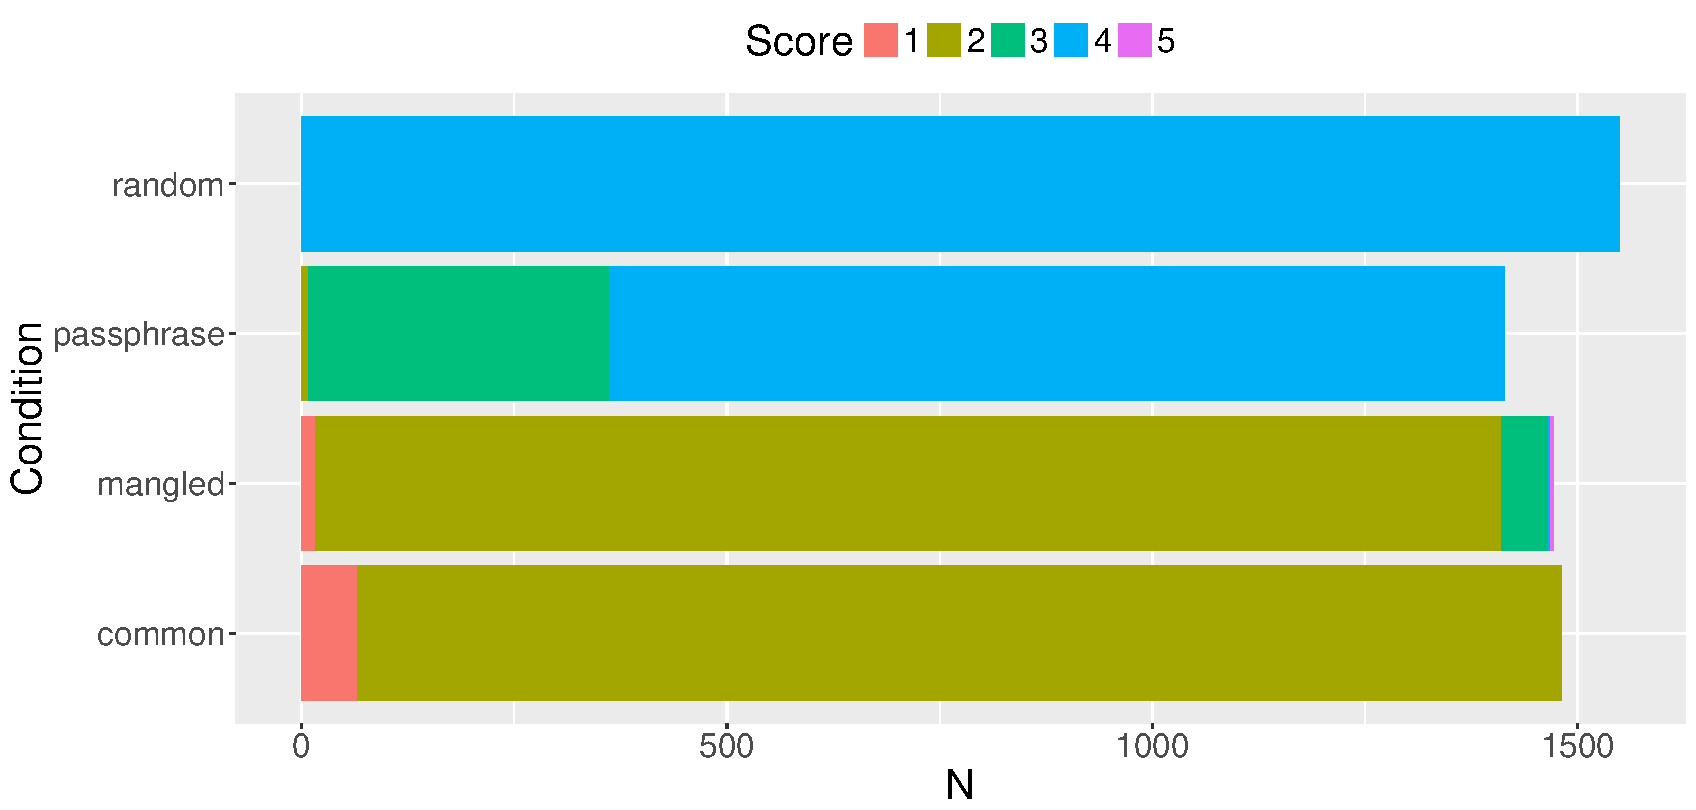
\includegraphics[width=0.9\linewidth]{pasdjo/score-distribution-all}
	\caption{\label{fig:pasdjo:zxcvbn-score-distribution} Distribution of zxcvbn scores for N=5915 passwords collected in the first four months of deployment (1 = weak, 5 = strong). Random passwords were the most stable condition with consistent score of 4. Mangled passwords show a range of 1 to 5, but passphrases were least predictable.}
\end{figure}

Moreover, from the distribution in Figure \ref{fig:pasdjo:zxcvbn-score-distribution} we can observe that in most cases, the maximum deviation $D_{max}$ less than 4: $D_{max} = 3$ in 5420 cases, and $D_{max} = 2$ in 410 cases. In other words, the user's estimate deviates by \textit{at most} 3 score points in 98.56\% of cases. At the same time, it is difficult to \textit{under}estimate passwords that had already received a low score. This narrows interval of the expectancy value for common and mangled passwords, i.e. users are more likely to \textit{over}estimate these -- if at all. These two findings motivate taking the absolute value of the deviation and create an overall accuracy score for each game played, just like we did. 

%What data did we throw out and why (known accounts)? how much of the dataset is that?

\subsubsection{``First Game'' Statistics}
A player's first game is vital for the assessment of their pre-existing strength perceptions in different conditions. After the first game, learning effects induced by our feedback are likely to change their subsequent judgments. Therefore, the first game is the most valuable indicator of mental models of password strength. In their first game, players achieved an average score of 2010 points (SD=653.16, Min=350, Max=3675), which translated to an average accuracy of 74.58 per cent of the achievable points. Moreover, players rated 27.21 passwords in their first game (SD=8.34), which is more than in subsequent games, albeit not significantly ($t_{32}(2) = 1.13, p > 0.1, 95\%-CI = [-2.04;7.12]$).%created with JASP (first-vs-sub-rounds-played.csv)
The first games consisted of 6.9 Common (25.3\%), 6.8 Mangled (25\%), 7.2 Random passwrods (26.5\%), and 6.3 Passphrases (23.2\%). The conditions were thus evenly distributed (\statsgt{3}{2.36}{0.05}). 

%\paragraph{Accuracy Breakdown}
As a next step, we can evaluate the achieved accuracy for each player in each condition. Since four users of did not rate at least two passwords in each condition, we remove their data and maintain a sample of N=111 users. Non-parametric tests are used to account for the coarse password ratings (1 through 5). 

\begin{figure}[tbp]
	\centering
	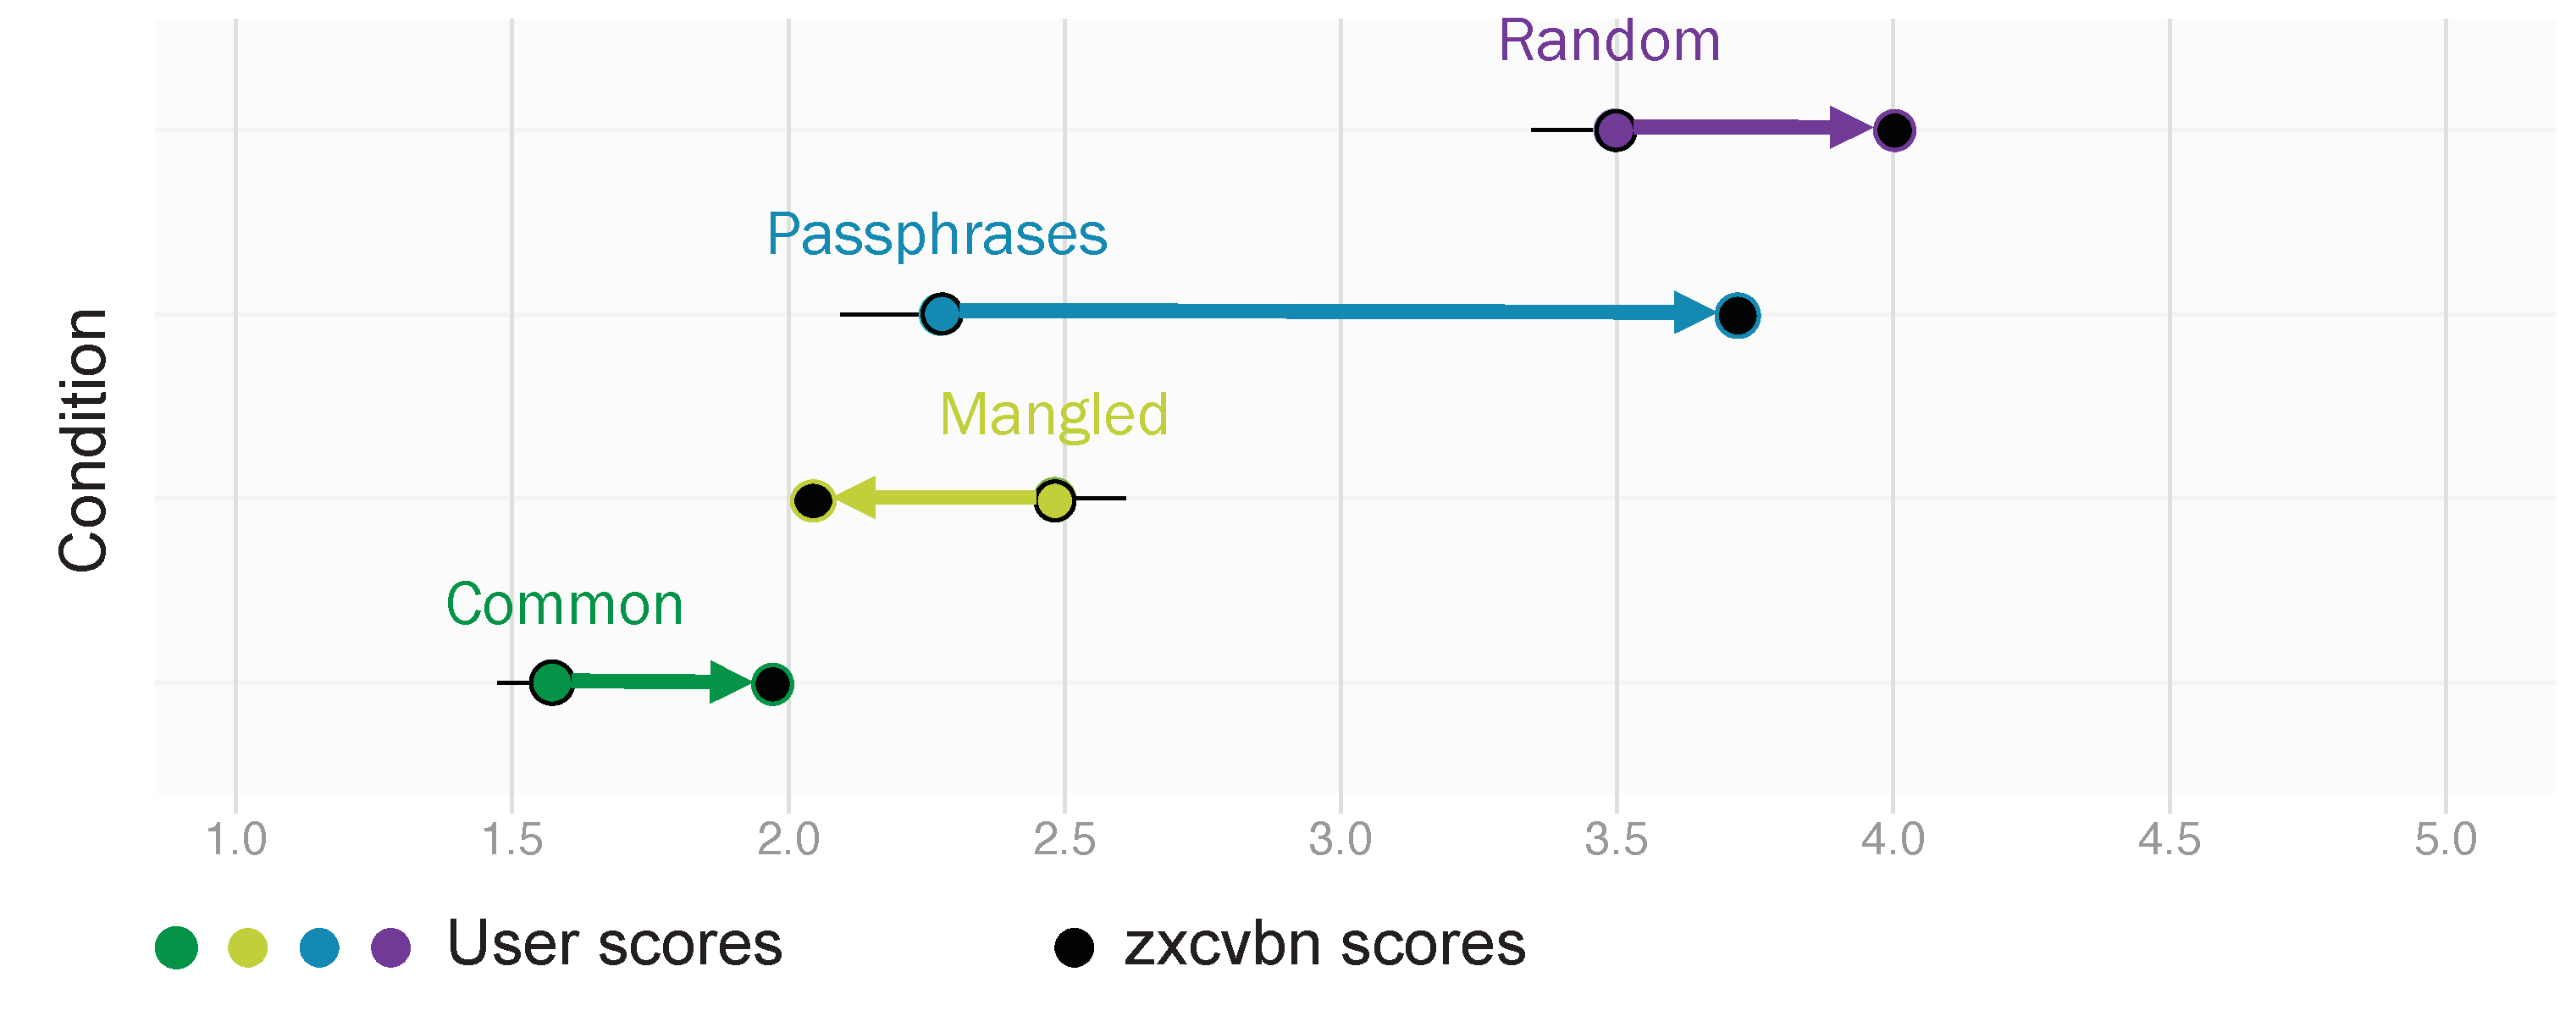
\includegraphics[width=\linewidth]{pasdjo/deviation-viz}
	\caption{\label{fig:pasdjo:deviation-viz} Average user ratings in each of the four conditions, plotted alongside mean zxcvbn scores. Users' estimations were least accurate for passphrases, which they had rated 1.4 points lower than zxcvbn. (N=111) }
\end{figure}

In their first game, players showed fairly consistent inaccuracies (see Figure \ref{fig:pasdjo:deviation-viz}) . Mangled passwords were the only condition that was overestimated (estimated median deviation $Md=0.5$). Interestingly, common passwords were underestimated slightly, although there was little room for underestimation ($Md=-0.5$). Random passwords were also underestimated by about half a point ($Md=-0.5$). The users in this data set rated passphrases exceptionally low ($Md = -1.6$). A Friedman rank-sum test showed significant significant differences for the deviations across the four conditions (\statslt{3}{187.84}{0.001}). We followed up this finding with Bonferroni-corrected post-hoc tests, i.e. $\alpha_{Bonf}=0.008$. Wilcoxon paired sample tests revealed significantly different deviations between all pairs of conditions, except for the common/random pair. In other words, common and random passwords were equally inaccurately assessed by the users. 

\subsubsection{Score Development}
From the 115 users who finished one game, 33 kept on playing for at least one more game. We tried to model their progress through a linear regression with gameIndex as predictor and achieved percentage as dependent variable. To account for the fact that some users played more rounds per game, we weighted the percentage with the number of passwords rated in that game. The model shows that players were able to improve their accuracy by playing multiple times (F(1)=49.37, \pvallt{0.001}, $\beta$ = 0.54, $R^2_{adj}$ = 0.23). Figure \ref{fig:pasdjo:percent-evolution} visualizes the progress of users who played at least twice. In there, it is also evident that the slope is not stringent, i.e. an individual user's accuracy does not necessarily increase steadily. We attribute this to the element of randomness in the game, which makes it more difficult in some cases to rate the passwords, while it might be easier in a subsequent game. 

\begin{figure}
	\centering
	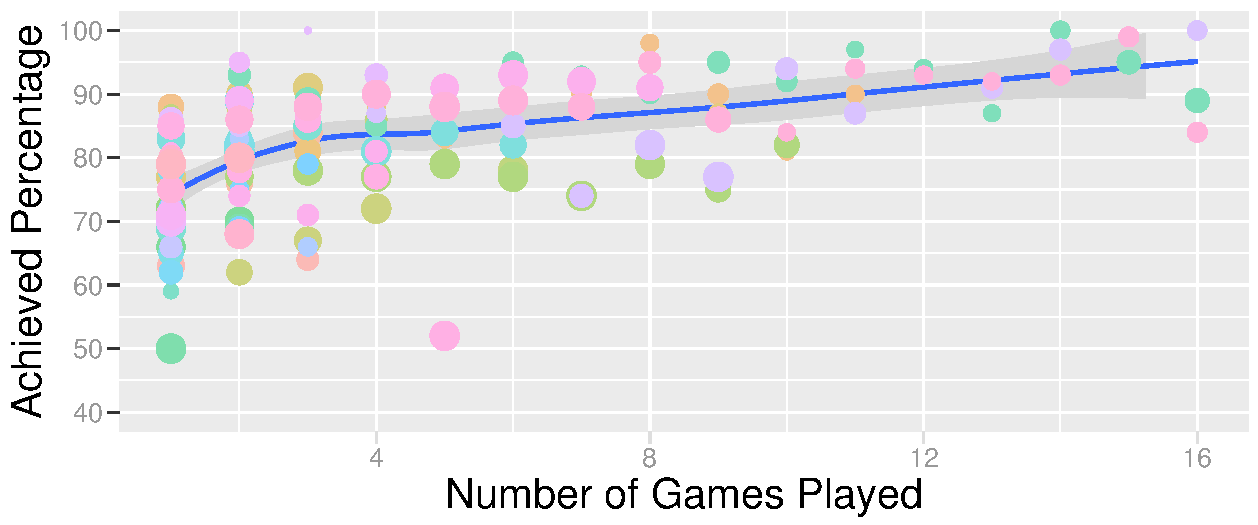
\includegraphics[width=\linewidth]{pasdjo/percent-evolution-reg-multi}
	\caption{\label{fig:pasdjo:percent-evolution} Achieved percentage (accuracy) evolution depending on the number of games played. Each dot represents a full game of a user, the size of the dot indicates how many passwords were rated in that particular game. Although a linear model works, we used a locally weighted polynomial regression (LOESS) to fit a line through the data points. Users clearly become better the more they play.}
\end{figure}

%here we report on the findings as discussed in the OzCHI paper.

\subsection{Extended Sample and Results}
\begin{figure}
	\centering
	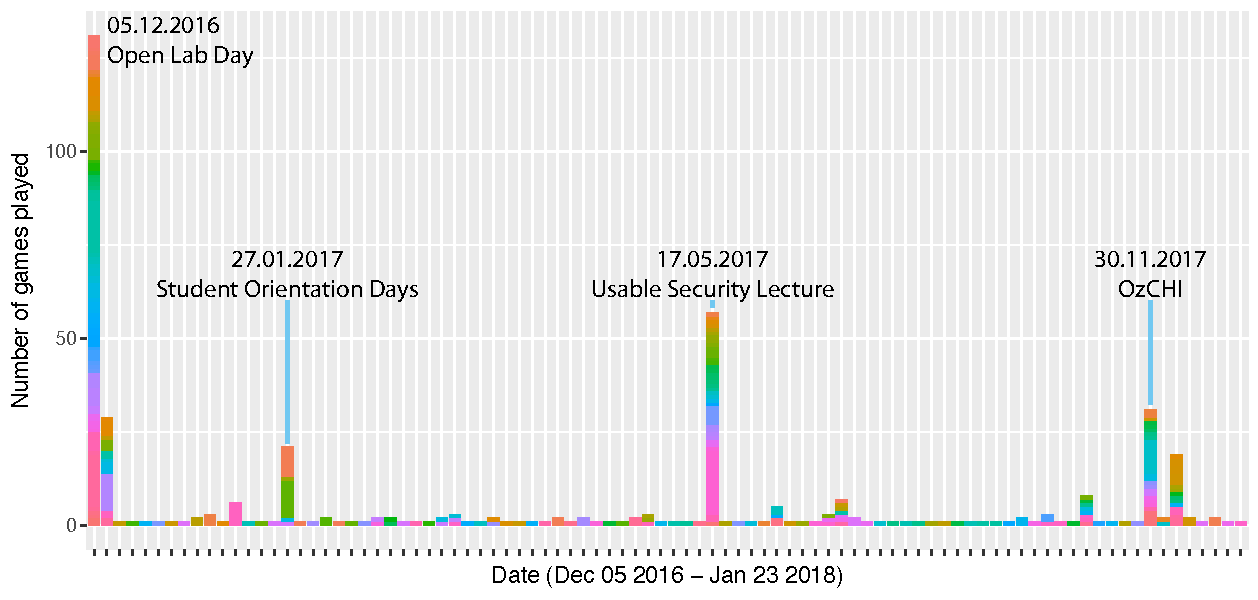
\includegraphics[width=\linewidth]{pasdjo/games-per-day-annotated}
	\caption{\label{fig:pasdjo:games-1y} The game was played on 90 distinct days (days with 0 games are not shown in the graph). There were four major drivers for the adoption (see annotations), that indicate that the sample mostly consists of students, their peers, and other academics.}
\end{figure}

On the 23rd of January, I created a new data dump and re-ran the analyses to see whether there were any differences to the first publication. The data set at this point consisted of 10,965 played rounds from 342 games played by 190 users on 90 distinct days (see Figure \ref{fig:pasdjo:games-1y}). Thus, there was an increase in 41.32\% in terms of games, and 85.38\% of played rounds. Before we look at the logs, we briefly present the changes introduced in PASDJO v2, which was deployed on November 7th 2017 (i.e. prior to the OzCHI conference, where the game was demoed)

\subsubsection{Version 2}
After publishing the first results, I had iterated the design and implementation of the game. There were a number of changes that might affect the players' performance. Splitting the data between v1 and v2 allows us to compare the players' performance before and after the adjustments to measure their effectiveness. 

\paragraph{New Condition: Predictable} The mangled passwords were algorithmically altered versions of common passwords. This often made it hard to figure out the original password. Perhaps, the mangled passwords sometimes seemed more like random passwords which is why they were the only overestimated condition in the first sample. The new condition ``Predictable'' mimicks the most predictable user alterations. The resulting passwords consist of a capitalized dictionary word with a predictable suffix, e.g. `123' or `!'. There were 12 predefined suffixes, and they were randomly appended to the dictionary word. 

\paragraph{Tuning Password Generation} After realizing that virtually no passwords had received a score of 5 in the first sample, I fine-tuned the generation of passphrases and random passwords. Passphrases were now either two or three words. Separators (e.g. a dash ``-'') were inserted in between the words. Random passwords used to be ten characters long in version 1. In version two their length is also randomized between 7 and 15 characters. This leads to a higher variety of zxcvbn scores. The resulting passwords sometimes resemble the mangled condition, which is a greater challenge for the players. Moreover, we increased the likelihood of common passwords from the top 100 by a factor of two. All measures resulted in a much more diverse spectrum of scores as shown in Figure \ref{fig:pasdjo:score-distribution-v2}.

\begin{figure}[htbp]
	\centering
	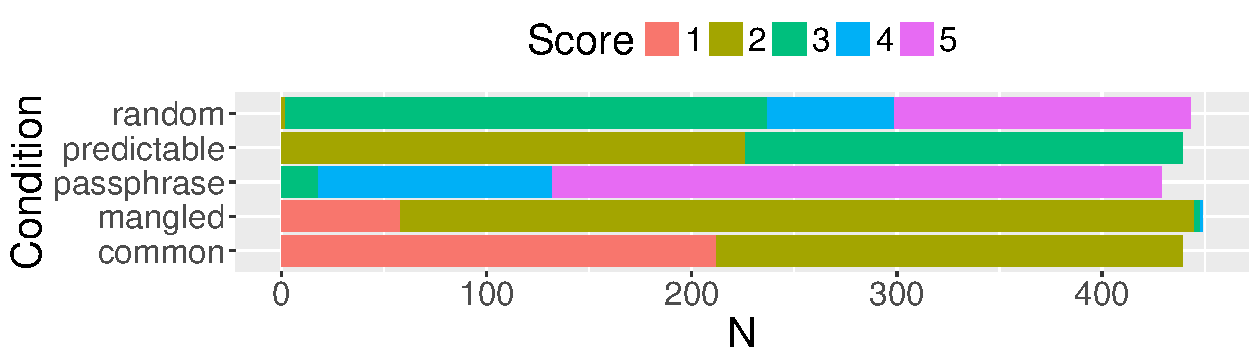
\includegraphics[width=0.7\linewidth]{figures/pasdjo/score-distribution-v2}
	\caption{\label{fig:pasdjo:score-distribution-v2}Zxcvbn scores in version 2. The scores within the conditions had become much more diverse, which should make it more difficult for players to judge individual passwords.}
\end{figure}

\paragraph{Scoring and Feedback} The players' achieved score ($A$) did not entirely reflect their performance. For instance, if a player rated as many passwords as possible without spending much thought on the strength, they still achieved a high score, albeit not a high accuracy. Therefore, the accuracy is now used as a ``penalty'' by multiplying the achieved score with the accuracy (e.g. $3000A~*~0.5P=~1500$ final score), which represents the performance much more adequately. Furthermore, the players had to figure out why their ratings deviated from the zxcvbn scores on their own. Now, the feedback screen contains a small indication as to how the score was calculated. This enables players to improve their score in the next game. 

\paragraph{Leaderboard and History} Finally, we introduced a new game-design element, namely leaderboards. Players can pick an alias and submit their score after each game. The main purpose of the leaderboard is to encourage \textit{competition}, which is another persuasive design strategy. 

%%%% SCORE DEVELOPMENT V2
\subsubsection{Score Development}
\begin{figure}[htbp]
	\begin{subfigure}[t]{0.49\linewidth}
		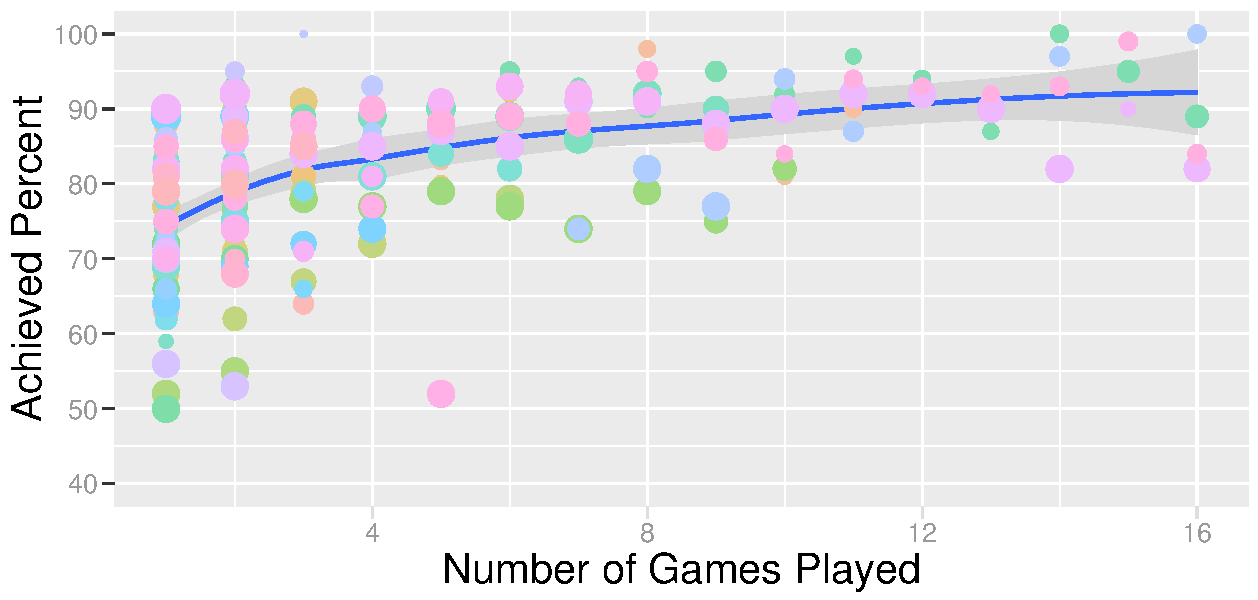
\includegraphics[width=\textwidth]{pasdjo/player-progress-multiplayers}
		\caption{\label{fig:pasdjo:1y-progress}Performance of players (Dec 2016 - Jan 2018)}
	\end{subfigure}
	\begin{subfigure}[t]{0.49\linewidth}
		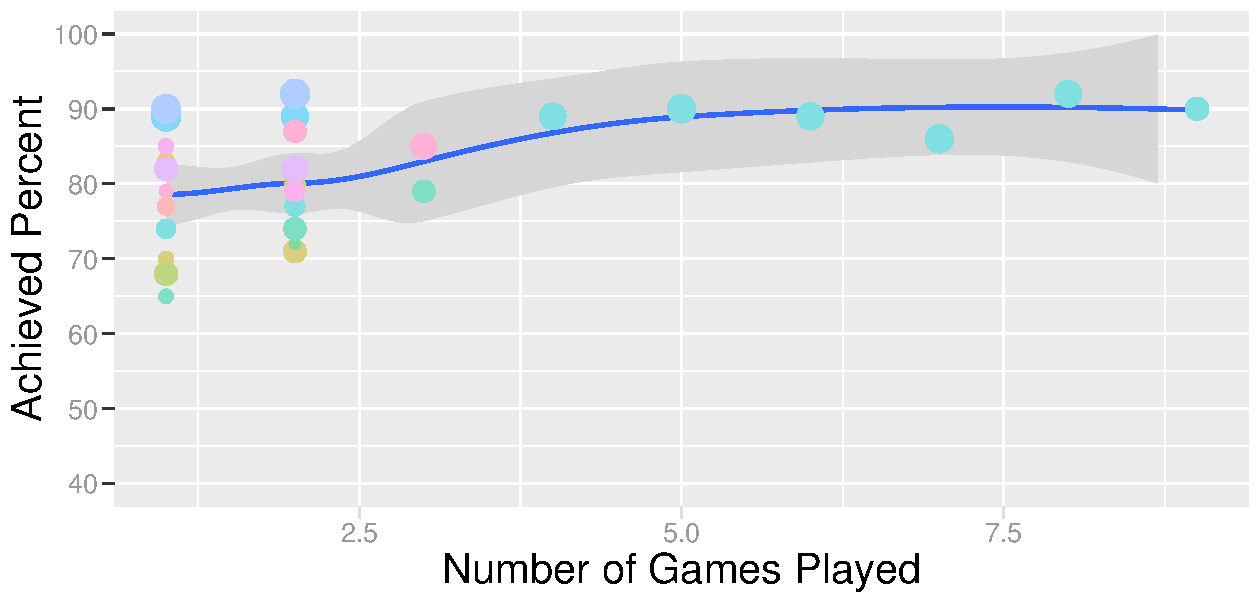
\includegraphics[width=\textwidth]{pasdjo/v2-player-progress-multiplayers}
		\caption{\label{fig:pasdjo:v2-progress}Performance of version-2 players}
	\end{subfigure}
	\caption{\label{fig:pasdjo:v2-progess-comparison} Performance development during the first 13 months of public deployment (\ref{fig:pasdjo:1y-progress}). In November 2017, version 2 was released, which roughly shows a similar learning curve.}
\end{figure}
Among the players who played at least two games, the overall score development has not changed visibly (see Figure \ref{fig:pasdjo:1y-progress}), with no notable differences in the regression model 
(F(1)=67.12, \pvallt{0.001}, $\beta$ = 0.53, $R^2_{adj}$ = 0.23). However, if we look at the players who played version 2, we can observe a slight decrease in the model fit (F(1)=8.83, \pvallt{0.01}, $\beta$ = 0.43, $R^2_{adj}$ = 0.20): There were 12 players who played version 2 more than once ($M=2.9, SD=2.29$). Their progress is shown in Figure \ref{fig:pasdjo:v2-progress}. The decrease can be explained by the fact that only one player played more than three times in this reduced data set. %another user scored really really hight in their first game already, distorting the model 

%%%%%%%% Strength perceptions
\subsubsection{Strength Perception in the First Game}
We also re-calculated the users' average accuracy in each condition, again only using the players that had generated data in all conditions in their first game (see Figure \ref{fig:pasdjo:v1-v2-deviations}). As before, the deviations from the zxcvbn scores differed significantly across conditions in version 1 (\statslt{3}{316.4}{0.001}). The same goes for version 2 of the game ((\statslt{4}{108.7}{0.001})). All post-hoc pairwise comparisons showed significant differences \pvallt{0.008} for version 1. For version 2, the situation is not as clear, because the sample is smaller (724 observations). The significantly different pairs were Mangled-Common, Mangled-Passphrase, Mangled-Predictable, Mangled-Random, Passphrase-Common, Passphrase-Predictable, Passphrase-Random \pvallt{0.005}. The lack of significant pairwise comparisons is also visible in Figure \ref{fig:pasdjo:v2-performance}: The users' ratings did not deviate much from the zxcvbn score in both the Common and the Random condition, which explains this result. In other words, mangled and predictable passwords as well as passphrases caused the players the most trouble, so their accuracy in these three conditions differed significantly. 
\begin{figure}[htbp]
	\begin{subfigure}[t]{0.49\linewidth}
		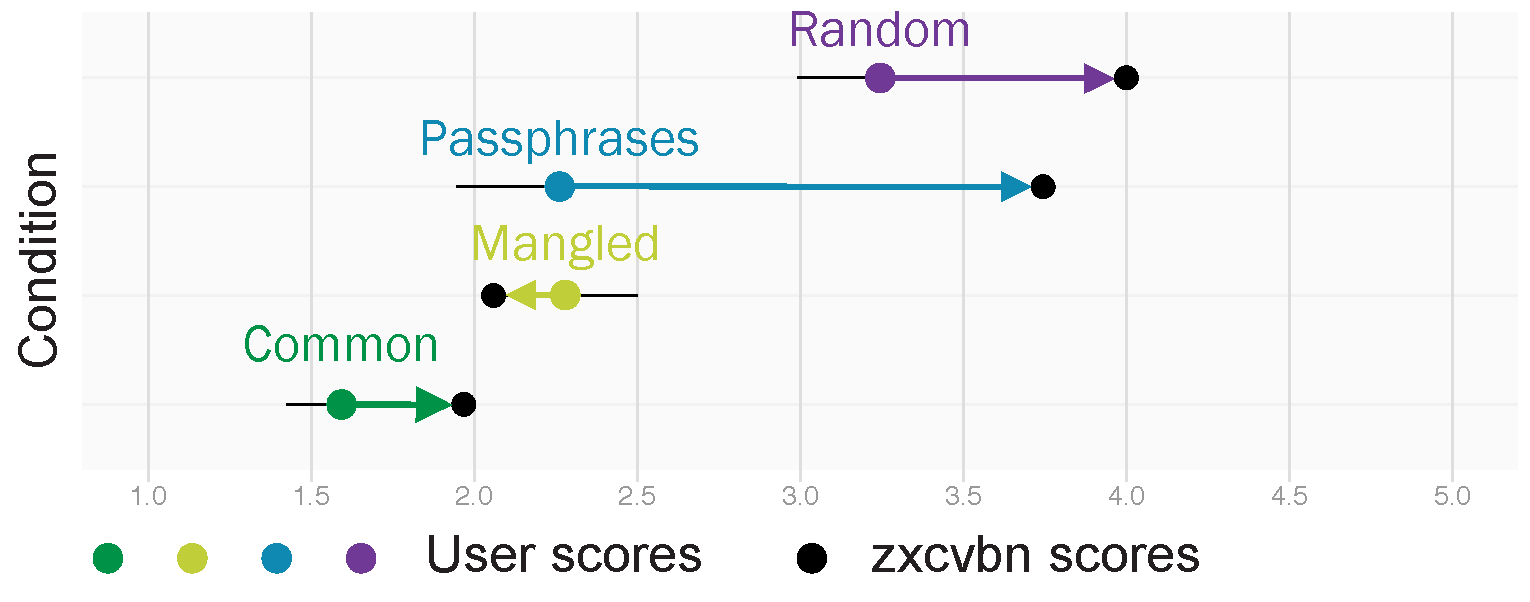
\includegraphics[width=\textwidth]{pasdjo/user-rating-v1-ci-annotated}
		\caption{\label{fig:pasdjo:1y-performance}Deviations of user ratings of v1 players (N=181)}
	\end{subfigure}
	\begin{subfigure}[t]{0.49\linewidth}
		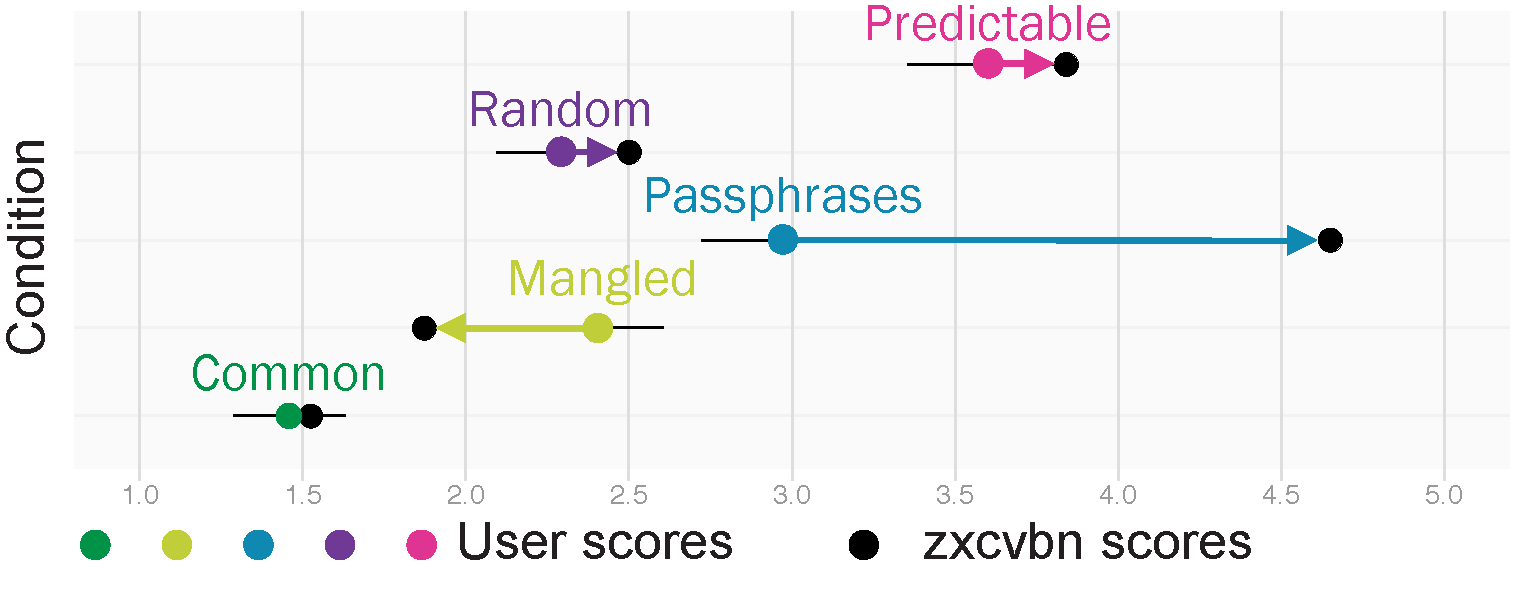
\includegraphics[width=\textwidth]{pasdjo/user-rating-v2-ci-annotated}
		\caption{\label{fig:pasdjo:v2-performance}Deviations of user ratings of v2 players.(N=52)}
	\end{subfigure}
	\caption{\label{fig:pasdjo:v1-v2-deviations} Users' average ratings, for PASDJO version 1 on the left and version 2 on the right. The version switch appears to boost accuracy for common and random passwords, but not for mangled passwords and passphrases.}
\end{figure}



\section{Discussion}
\subsection{Players' Overall Performance}
Overall, we can attest players a fairly good performance. This assessment resounds to Ur \etal's results \cite{Ur2016PerceptionsPassword}. Players performed best in the ``Common'' condition, i.e. they can identify commonly used passwords with high certainty. Algorithmically mangled -- but common! -- passwords caused a bit more trouble. The fact that this was the only condition where people judged strength as too high reveals the users' mental model: \textit{if one substitutes individual letters with digits and symbols, the password must become stronger}. The additional data for version 1 helped narrow down the confidence intervals and moving closer to the ``actual truth''. After about one year, the average rating for mangled passwords had moved closer to the zxcvbn score (compare Figures \ref{fig:pasdjo:deviation-viz} and \ref{fig:pasdjo:1y-performance}). Perhaps this means that the players that followed ($\delta(n)=70$) had a better mental model of the implications of character substitutions. However, since none of the other average ratings changed significantly, the shift might be due to chance. 

\subsection{Strength Perception vs. Selection}
- the data shows strong similarities to Ur \etal \cite{Ur2016PerceptionsPassword}
- perception and estimation of password strength appear to be easy for the players of our games even if they might not have a background in cyber security. 
- you rarely see passwords of other people, only when they share it with you. In many cases passwords that are shared with you are typically not the strongest passwords \cite{Haque2014Hierarchy,  Shay2010EncounteringPasswordRequirements, Singh2007PasswordSharing, Violettas2014PasswordsAvoidGreece, Weirich2001PrettyGoodPersuasion, ZhangKennedy2016RevisitingPasswordRules} 

\subsection{Intuition}
The time pressure and lead to users only spending 2.45 seconds on average per password. Can we assume that this indicates System 1 responded?

\subsection{Passphrases}
% passphrases were hard to estimate. 
If you correctly identify a passphrase, you still need to count the number of characters to make a more informed decision about the strength estimation. The time pressure kept users from doing just that so we can safely assume that passphrases were rated very intuitively %TODO it would be possible to merge this section with the one above. 

% system generated passphrases vs user-generated passphrases.

\subsection{Changing users' mental models with PASDJO}
The learning effects clearly indicate that users learned assessing password strength after playing PASDJO. This makes us wonder if deploying such a game in different contexts, potentially in even shorter forms could effectively educate users. 

\subsection{Limitations}
We discussed the most important limitations regarding the methodology in Section \ref{sec:pasdjo:beneftis_shortcomings_method}. Therefore, we focus on the limitations in the data and test results in this section. 

% clustering of dates around events -- see figure with time line histogram
From Figure \ref{fig:pasdjo:games-1y}, it is evident that most games were played at special events at the university or at conferences. Therefore, we can safely assume that our sample consists mostly of students, their peers, and academics. Thus, we must be careful not to expect the same strength assessment from other user groups or larger populations. Nonetheless, many players in our one-year trial might not have a background in cybersecurity and thus, we are confident that the sample still represents a useful cross-section of a diverse enough population. Plus, the data was collected in the wild, which further increases its ecological validity. 

% version bump
Moreover, version 2 introduced a number of improvements that would have been nice-to-have already in the earlier version. Still, in the first version, the different conditions were easier to tell apart. Thus, causal effects are easier to isolate. 

% zxcbn!
Finally, the strength ratings in PASDJO are solely based on zxcbn scores. While it is a state-of-the-art metric (see Section \ref{sec:rw:zxcbn}), other metrics might model real-world attacks better in some situations. For instance, we could have chosen Melicher's JavaScript implementation of neural network strength estimation \cite{Melicher2016NeuralNetworks}. However, it is more challenging to integrate and also does not map password strength to a scale from 1 to 5, but to a guess number. The same goes for other estimators. Nonetheless, zxcvbn's assessments correlated strongly with the output from \gls{PGS}. Therefore, we are confident that zxcvbn is the best tool for the constraints of our game. In the future, it might be worthwhile use multiple strength metrics to obtain a more differentiated strength assessment.

\section{Summary}
\begin{itemize}
	\item users performed better than anticipated
	\item misconceptions mainly involve passphrases and mangled passwords (and predictable alterations!). common passwords were confidently identified. 
	\item the game was updated after the first results were in and is still deployed. Google even uses it internally. 
	\item the source code is available on GitHub \footurl{https://github.com/TobiasSeitz/pasdjo}{24.01.2018}.
	\item contribution: longitudinal data.
\end{itemize}


\subsection{Future Work}
Better onboarding
Challenges
Player Profiles 
adding the game to password management software


\subsubsection{Take-Aways}



